% vim:tw=78:ai:bg=light:set spell:spelllang=de:set nu
%%%%%%%%%%%%%%%%%%%%%%%%%%%%%%%%%%%%%%%%%%%%%%%%%%%%%%%%%%%%%%%%%%%%%%%%%%%%
%%% Ultraschall
%%%%%%%%%%%%%%%%%%%%%%%%%%%%%%%%%%%%%%%%%%%%%%%%%%%%%%%%%%%%%%%%%%%%%%%%%%%%
\chapter{Ultraschall}
Die Ultraschalllokalisation benutzt die Laufzeit von Schallsignalen um
Entfernungen zu bestimmen. Um aus Entfernungen Rückschlüsse auf eine
Position ziehen zu können, werden mehrere verschiedene Strecken und Längen
benötigt. Aus diesen kann mit Hilfe der Triangulation ein Objekt lokalisiert
werden. Dabei gibt es im wesentlichen zwei Ansätze. Zum einen gibt es den
Ansatz, der \dq Sprechenden Infrastruktur\dq, bei dem das zu lokalisierende Objekt
einen Empfänger darstellt, der Signale von Beacons aufnimmt. Der andere
Ansatz ist genau umgekehrt, man spricht von \dq Sprechenden Knoten\dq.

\section{Sprechende Infrastruktur}
Wie der Name schon andeutet, wird bei diesem Verfahren ein System verwendet,
welches von vielen Stellen Ultraschallimpulse in der Raum sendet. Zusätzlich
wird ein RF-Signal von jedem Beacon ausgesandt, das den Zeitpunkt des
Absendens eines Ultraschallimpulses und das Muster des Impulses beinhaltet.
Da RF-Signale signifikant schneller sind als Ultraschallimpulse, weiß das
Objekt über den eintreffenden Ultraschallimpuls schon bescheid, bevor dieser
eintrifft. Auf Grund der Kenntnis des Absendezeitpunktes des
Ultraschallimpulses kann somit die Entfernung des Objekts zum Beacon
berechnet werden.

Um eine ausreichend genaue Lokalisation zu erzielen, müssen viele dieser
Beacons installiert werden. Durch Trilateration kann aus den bekannten
Koordinaten der Beacons und der gemessenen Entfernungen die Position
bestimmt werden.

Ein sehr bekanntes System nennt sich Cricket, welches am Massachusetts
Institute of Technology entwickelt
wurde. Cricket erreicht eine Genauigkeit von 1-2 cm auf 10 m Entfernung.
Die Cricket-Einheit kann sowohl als Beacon, als auch als Empfänger
konfiguriert werden und arbeitet mit einer Updaterate von einem Hz.

\section{Sprechender Knoten}
Das System des \dq sprechenden Knotens\dq{} arbeitet im Gegensatz zu dem der
\dq Sprechenden Infrastruktur\dq{} nach dem umgekehrten Prinzip. Die
Hauptrolle spielt hierbei ein bewegter Beacon der kontinuierlich
Ultraschallimpulse erzeugt. Das Gegenstück ist ein Netzwerk von sehr präzise
positionierten Empfängern, die das Signal des Beacons auffangen. Die
Berechnung der Position wird hier im Grunde genauso bestimmt wie bei der
\dq Sprechenden Infrastruktur\dq{}, es wird die Zeit gemessen, die der
Ultraschallimpuls vom Beacon zum Empfänger braucht. Durch die vielen
Empfänger lässt sich sehr gut eine 3D-Position bestimmen.

Ein Vorreiter auf diesem Gebiet ist das \dq Active Bat\dq -System. Seine
Genauigkeit bei der Lokalisierung liegt bei 2 cm und im 3D-Bereich bei 5 cm.

\section{Unterschied}
Der Unterschied der beiden Methoden ist, wo die Berechnung der Lokalisation
statt findet. Die Methode \dq Sprechende Infrastruktur\dq{} eignet sich dabei
sehr gut, um einen bewegten Empfänger die Möglichkeit zugeben sich selbst in
einer entsprechenden Umgebung zu Lokalisieren. Bei der Methode
\dq Sprechender Knoten\dq{} wird die Berechnung jedoch außerhalb des bewegten
Objektes vorgenommen. Damit kann ein sendendes Objekt in einem dafür
ausgestattetem Raum lokalisiert werden.

\section{Triangulation}
Da die Schallgeschwindigkeit bekannt ist, kann über die Laufzeit des
Ultraschallimpulses die Entfernung zwischen dem Beacon $O$ und den
Empfängern $S_1$ und $S_2$ berechnet werden. Wenn wir von 20 $^\circ$C warmer
Luft ausgehen, beträgt die Schallgeschwindigkeit somit 343 m/s. Die Entfernung
kann mit Hilfe des Gesetzes für die gleichförmige Bewegung berechnet werden.

\begin{equation}
  d = v\cdot t
\end{equation}

Dabei ist $d$ die Entfernung zwischen dem Beacon $O$ und dem Empfänger,
$v$ die Schallgeschwindigkeit und $t$ die Impulslaufzeit.

Allerdings kann mit einer gemessenen Entfernung, nicht die genaue Position des
Beacons bestimmt werden. Mit einer zweiten Entfernung
kann jedoch die Position über eine Dreiecksbildung bestimmt werden.
Dieses Problem wird in Abbildung 2.1 dargestellt.

\begin{figure}[htbp]
  \centering
  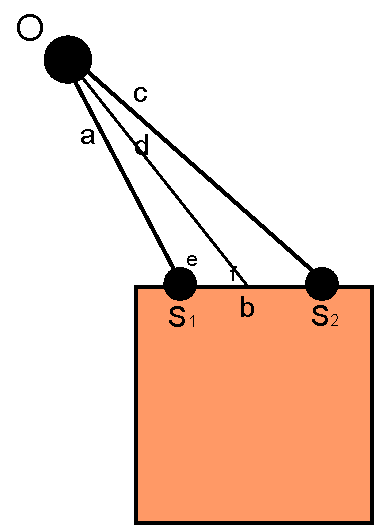
\includegraphics{figures/triangulation.pdf}
  \caption{Triangulation}
\end{figure}

Die beiden Empfänger $S_1$ und $S_2$ mit dem Abstand $b$, nehmen jeweils eine
Entfernung zum Beacon $O$ wahr. Je nachdem, welche der beiden
Entfernungen $a$ oder $c$ größer ist, kann entschieden werden, ob
sich der Beacon links oder rechts der Hauptachse der Empfänger
befindet. Um nun die tatsächliche Entfernung $d$ von der Mitte der
Sensoren und den genauen Winkel $f$ zum Beacon zu berechnen, kann der
Kosinussatz verwendet werden.

\begin{equation}
  c^2 = a^2 + b^2 - 2ab\cdot cos(\gamma)
\end{equation}

Zunächst wird der Winkel $e$ berechnet.

\begin{equation}
  e = acos\left(\frac{c^2 - a^2 - b^2}{-2ab}\right)
\end{equation}

Mit dem Winkel $e$ kann nun die exakte Entfernung $d$ von den Empfängern
zum Beacon berechnet werden.

\begin{equation}
  d = \sqrt{a^2 + \left(\frac{b}{2}\right)^2 - 2ab\cdot cos(e)}
\end{equation}

$f$ ist der Peilungswinkel von der Empfängerhauptachse zum Beacon. Der
Peilungswinkel gibt an, um wie viel Grad sich die Position des Beacons ändern müsste,
um genau Senkrecht zu den Empfängern zu stehen. Er lässt sich ebenfalls durch
den Kosinussatz berechnen.

\begin{equation}
  f = acos\left( \frac{a^2 - \left(\frac{b}{2}\right)^2 - d^2}{-bd} \right)
\end{equation}

Mit diesen beiden Werten $f$ und $d$ ist es jetzt möglich, die genaue
Position des Beacons zu bestimmen.

Diese Rechnung ist nur ein Beispiel dafür, wie Triangulation funktioniert.
Zwei Entfernungen reichen natürlich nicht aus, um eine ausreichende
Lokalisierung zu erhalten.

\section{Probleme}
Die Ultraschalltechnologie hat jedoch ein paar starke Nachteile. Die
Schallgeschwindigkeit ist abhängig von der Lufttemperatur. Bei der
Laufzeitmessung der Signale muss das berücksichtigt werden, indem eine
zusätzliche Information über die Temperatur mitgesendet werden muss. Das
wiederum macht den Aufbau des Senders oder Empfängers aufwendiger, da diese
mit einem Temperatursender ausgestattet werden müssen. Eine weitere
Möglichkeit wäre die Temperaturen separat zu messen und über ein Datennetz
zu verteilen.

Ein weiteres Problem sind Reflexionen der Ultraschallimpulse an glatten
Wänden. Es entstehen \dq Multipfadsignale\dq{} die den Empfänger verwirren
können. Es muss sichergestellt werden, dass die Signale zugeordnet werden
können. Zum Beispiel mit einem mitgesendeten RF-Signal.

Des Weiteren besteht die Möglichkeit, dass Ultraschallimpule verdeckt werden.
Wenn sich ein Beacon in meinem Raum mit vielen Störquellen befindet, z.B.
Menschen oder großen Geräten, kann es passieren, dass Impulse verloren gehen,
weil sie vorher von einem anderen Objekt absorbiert wurden. Um dem zu
begegnen, wäre es denkbar, den Bewegungspfad zu Interpolieren und durch
Messungen zu korrigieren. So fällt ein Ausfall nicht groß ins Gewicht.

\section{Vorteile}
Ein großer Vorteil in der Nutzung von Ultraschall ist die bereits sehr gute
Erforschung. Es gibt sehr viele Untersuchungen zu den verschiedensten
Aspekten. Ultraschallsender und Empfänger sind darüberhinaus auch nicht so
Kostenintensiv wie z.B. Laser oder besonders hochwertige GPS-Empfänger für
Indoor-Applikationen. Der Aufwand, um aus den Laufzeitdaten eine Position zu
berechnen ist zu dem viel geringer als z.B. die der Lokalisation durch
Funksignalstärke.

%%%%%%%%%%%%%%%%%%%%%%%%%%%%%%%%%%%%%%%%%%%%%%%%%%%%%%%%%%%%%%%%%%%%%%%%%%%%
\cleardoublepage
